\documentclass[12pt,a4paper]{article}
\usepackage[utf8]{inputenc}
\usepackage[russian]{babel}
\usepackage[OT1]{fontenc}
\usepackage{mathtools}
\usepackage{amsfonts}
\usepackage{amssymb}
\usepackage{enumitem}
\usepackage{alltt}
\usepackage{graphicx}
\usepackage{indentfirst}
\usepackage{caption}
\usepackage{float}
\usepackage{wrapfig}
\setlength{\parindent}{0.75cm}
\graphicspath{{pictures/}}
\DeclareGraphicsExtensions{.png}
\usepackage[left=15mm,right=15mm,top=2cm,bottom=2cm]{geometry}
\author{Глотов Алексей}
\begin{document}
\newpage
\begin{center}
\footnotesize{{ГОСУДАРСТВЕННОЕ АВТОНОМНОЕ ОБРАЗОВАТЕЛЬНОЕ УЧРЕЖДЕНИЕ}\break
{ВЫСШЕГО ОБРАЗОВАНИЯ}
\break
{\bf {МОСКОВСКИЙ ФИЗИКО-ТЕХНИЧЕСКИЙ ИНСТИТУТ}}
\break
\small{(НАЦИОНАЛЬНЫЙ ИССЛЕДОВАТЕЛЬСКИЙ УНИВЕРСИТЕТ)}}
\break
\hfill \break
\hfill \break
\begin{center}
\Large{Кафедра физической механики }
\end{center}
\hfill \break
\hfill \break
\hfill \break
\hfill \break

\begin{center}
\Large {Лабораторная работа 1}
\end{center}
\hfill \break\\
\large{Измерение температуры пламени методом обращения спектральных линий}
\end{center}
\hfill \break
\hfill \break
\hfill \break
\hfill \break
\hfill \break
\hfill \break
\hfill \break
\hfill \break
\hfill \break
\hfill \break

\begin{flushright}
{Работу выполнили:}

Волошиновский Даниил

Вострикова Станислава

Глотов Алексей
\end{flushright}

\hfill \break
\hfill \break
\hfill \break
\hfill \break
\hfill \break
\hfill \break
\hfill \break
\hfill \break
\hfill \break
\hfill \break
\hfill \break

\begin{center}
Долгопрудный \break
 2023
\end{center}
\thispagestyle{empty}
\newpage
\section{Введение}

\par В связи с актуальными задачами науки и техники необходимо производить измерения температуры излучающих тел и радиационных тепловых потоков от них. Обычные контактные методы являются мало пригодными из-за возникающей попутно задачи конвективного теплообмена. На первое место выдвигаются оптические методы измерения. Главными преимуществами этих методов является то, что они не требуют непосредственного контакта с измеряемым объектом и не вносят искажений в его параметры. 
\par В данной работе измерения температуры нагретых тел производятся двумя способами: пирометрическим, с помощью которого определяется температура раскаленных металлов, и методом обращения спектральных линий, с помощью которого определяется температура пламени пропановой горелки

\subsection{Теоретические сведения}

\par Введем понятие \textit{спектральной интенсивности излучения}  как количество энергии, переносимой излучением через площадку единичной площади, нормаль которой составляет угол $\phi$ с направлением распространения излучения за единицу времени, в единичном спектральном интервале длин волн, в единичном телесном углу. Тогда энергия, прошедшая через площадку $dS$ за время $dt$, составит

\begin{equation}
dU = I_{\lambda}\cos(\phi)dS{\times}d{\lambda}dtd\Omega
\end{equation}

\par Если считать, что выбранная площадка $dS$ расположена на поверхности излучающей среды, температура которой равна T, то интенсивность излучения с этой поверхности называется \textit{лучеиспускательной способностью поверхности тела} или \textit{спектральной поверхностной плотностью излучения в направлении нормали} и обозначается $E_{\lambda}(T)$

\par В случае изотропного, или диффузного, излучения с поверхности $dS$ энергия, излучаемая за время $dt$ внутри телесного угла $d\Omega$ в интервале длин волн $d\lambda$ равна

\begin{equation}
dU = E_{\lambda}(T)\cos(\phi)d{\lambda}dSd{\Omega}dt
\end{equation}  
- закон Ламберта (1760 г.)

Проинтегрировав по телесному углу в сферических координатах, получим:

\begin{equation}
\frac{U}{dt} = K_{\lambda}(T)dSd\lambda = E_{\lambda}(T)dSd\lambda\int_0^{2\pi}d\psi\int_0^{\pi/2}\sin{\phi}\cos(\phi)d\phi = {\pi}E_{\lambda}(T)dSd\lambda
\end{equation}

$K_{\lambda}(T)$ - \textit{полусферическая спектральная поверхностная плотность потока излучения}. 

\par Когда некоторое излучение $I_{\lambda}^0$ падает на тело, то можно рассмотреть несколько процессов. Часть излучения $I_{\lambda}^R$ отразится от тела. Та часть, которая пройдет в тело, может поглотиться (обозначим $I_{\lambda}^A$) и пройти без изменения ($I_{\lambda}^D$). Из закона сохранения энергии: 

\begin{equation}
I_{\lambda}^0 = I_{\lambda}^R + I_{\lambda}^A + I_{\lambda}^D
\end{equation}

\par Введем следующие понятия:
\begin{itemize}
\item $R_{\lambda} = I_{\lambda}^R/I_{\lambda}^0$ - спектральная \textit{отражающая} способность
\item $A_{\lambda} = I_{\lambda}^A/I_{\lambda}^0$ - спектральная \textit{поглощающая} способность
\item $D_{\lambda} = I_{\lambda}^D/I_{\lambda}^0$ - спектральная \textit{пропускательная} способность
\end{itemize}

\par Из этих определений и (4) следует:

\begin{equation}
R_{\lambda} + A_{\lambda} + D_{\lambda} = 1
\end{equation}

\par Если тело полностью поглощает падающее на него излучение произвольной частоты ($A_{\lambda} = 1$), то оно называется абсолютно черным телом. Его свойства лучше всего воспроизводит небольшое отверстие в замкнутой полости, стенки которой изготовлены из поглощающего вещества. Излучение, проникающее, через отверстие, почти полностью будет поглощено, следовательно, площадь сечения отверстия является поглощающей поверхностью черного тела. Если отверстие мало, то оно практически не влияет на излучение внутри полости. А если стенки полости изготовлены из однородного материала и поддерживаются при температуре T, то с течением времени установится равновесие поглощаемого и испускаемого излучения:

\begin{equation}
E_{\lambda}(T) + R_{\lambda}I_{\lambda}(T) = I_{\lambda}(T)
\end{equation}

\par Равновесное излучение, установившееся в полости, однородно и изотропно и характеризуется одной величиной - \textit{спектральной интенсивностью черного излучения} $B_{\lambda}(T)$. Таким образом: 

\begin{equation}
E_{\lambda}(T) = (1 - R_{\lambda}B_{\lambda}(T) = A_{\lambda}B_{\lambda}(T))
\end{equation}

откуда

\begin{equation}
\frac{E_{\lambda}(T)}{A_{\lambda}} = B_{\lambda}(T)
\end{equation}
- закон Кирхгофа (1898 г.)

\par Функция $B_{\lambda}(T)$ одинакова для всех веществ и ее можно определить теоретически. Это было сделано Планком в 1905 г.

\begin{equation}
B_{\lambda}(T) = \frac{2hc^2}{\lambda^5(e^{hc/{\lambda}kT}-1)}
\end{equation}

\par Чаще используется полусферическая спектральная поверхностная плотность излучения черного тела, равная ${\pi}B_{\lambda}(T)$. Для удобства приведем формулу (9) в следующий вид:

\begin{equation}
K_{\lambda}^p(T) = {\pi}B_{\lambda}(T) = \frac{C_1}{\lambda^5(e^{C_2/{\lambda}T}-1)}
\end{equation}
где $C_1 = 2{\pi}hc^2 = 3.74\cdot10^{-16}\text{Вт*м}^2, C_2 = hc/R = 1.44\cdot10^{-2}K$

\begin{figure}[h!]
	\begin{center}
		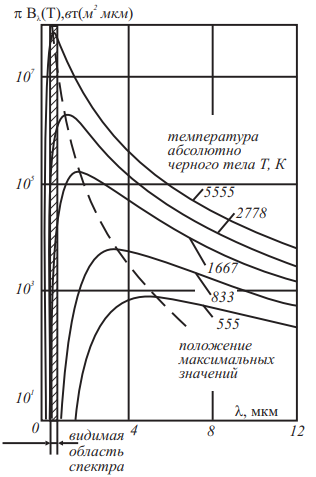
\includegraphics[width = 0.35\textwidth]{MSS-1-1}
		\caption{Зависимость спектральной полусферической плотности излучения черного тела от длины волны для нескольких значений температур}
	\end{center}
\end{figure}

\par Согласно закону распределения Планка, энергия, излучаемая одной стороной единичной поверхности во всем спектральном интервале:

\begin{equation}
N_S(T) = \int K_{\lambda}^p(T)d{\lambda} = \int_0^{\inf}{\pi}B_{\lambda}(T)d{\lambda} = \sigma_s{T^4}
\end{equation}
- закон Стефана-Больцмана, где $\sigma_s$ постоянная Больцмана
\begin{center}
$\sigma_s = \frac{12{\pi}^5k^4}{15c^2h^3} = 5.67\cdot10^{-8}\textbf{Вт/м}^2\cdot{K^4}$
\end{center}

\par \textit{Серое излучение}. Если все ординаты на рис. 1 уменьшить в одинаковое число раз, то получится спектральное распределение полусферической поверхностной плотности излучения, в точности подобное распределению интенсивности черного излучателя. Тело, для которого характерно такое распределение, называется "серым" излучателем. Величину 

\begin{equation}
\varepsilon_{\lambda}(T) = \frac{U_S(\text{истинная})}{U_S(\text{Стефан-Больцман})} = \frac{{\pi}E_{\lambda}(T)}{{\pi}B_{\lambda}(T)} = \frac{E_{\lambda}(T)}{B_{\lambda}(T)}
\end{equation}
характеризующую излучатель, назовем \textit{степенью черноты}

\begin{figure}[h!]
	\begin{center}
		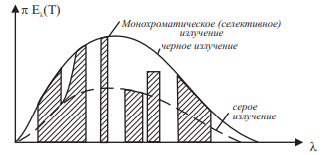
\includegraphics[width = 0.6\textwidth]{MSS-1-2}
		\caption{ Схематическое изображение
спектрального распределения интенсивности для черного, серого и селективного излучения.}
	\end{center}
\end{figure}

\par В данной работе нас будет интересовать спектральная степень черноты в направлении нормали

\begin{equation}
\varepsilon_{\lambda ,n} = \frac{E_{\lambda}(T)}{B_{\lambda}(T)}
\end{equation}
которая согласно закону Кирхгофа совпадает с определением поглощательной способности.

\subsection{Экспериментальная установка}

\par \textbf{Оптические методы измерения температуры реальных сред}
\par При достаточно высоких температурах металлы раскаляются и их температуру можно измерить, исследуя испускаемое ими излучение с помощью пирометров.

\par 
Работа пирометра основана на сравнении интенсивности света, излучаемого, с одной стороны, объектом, температуру которого измеряют, и, с другой стороны, фотометрической лампой накаливания
(с угольной или вольфрамовой нитью). В силу того, что спектральные характеристики объекта и нити накаливания пирометра могут отличаться, то уравнять визуально наблюдаемые интенсивности излучения объекта и нити во всем спектральном диапазоне чувствительности глаза невозможно. Поэтому применяется фильтр (как правило, красный с длиной волны порядка 0.65 мкм), для
вырезания достаточно узкого участка спектра излучения. Нить накаливания фотометрической лампы предварительно градуируют путем сравнения с излучением черного тела, температуру которого можно точно измерить в достаточно широком интервале.

\begin{figure}[h!]
	\begin{center}
		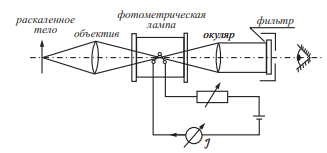
\includegraphics[width = 0.7\textwidth]{MSS-1-3}
		\caption{Пирометр с исчезающей нитью}
	\end{center}
\end{figure}

\par Так как параметры градуируются по излучению черного тела, то температура, определенная таким образом, равна температуре, которую имело бы черное тело с тем же тепловым излучением, что и излучаемый объект. Это называется яркостная температура $T_b$, она будет ниже истинной температуры T нагретого физического (нечерного) тела, степень черноты $\varepsilon_{\lambda ,n}(T)$ которого меньше единицы и, следовательно, тепловое излучение слабее. Так как измерение температуры основано на равенстве интенсивностей света, то можно записать:

\begin{equation}
I_{\lambda}(T) = B_{\lambda}(T_b)
\end{equation}
или 
\begin{equation}
\varepsilon_{\lambda ,n}(T)\frac{C_1}{e^{C_2/{\lambda}T}-1}=\frac{C_1}{e^{C_2/{\lambda}T_b}-1}
\end{equation}

\par Для температур, обычно получаемых в лабораториях, $C_2 \gg \lambda{T}$, с другой стороны, величина $\varepsilon_{\lambda ,n}(T)$ слабо изменяется в интервале температур $T \div T_b$, и поэтому ее можно заменить средним значением $\tilde{\varepsilon}_{\lambda ,n}(T)$. Тогда (15) запишем в виде

\begin{equation}
\tilde{\varepsilon}_{\lambda ,n}e^{-C_2/{\lambda}T}=e^{-C_2/{\lambda}T_b}
\end{equation}
откуда формула для определения истинной температуры тела

\begin{equation}
\frac{1}{T} = \frac{1}{T_b}+\frac{\lambda}{C_2}\ln \tilde{\varepsilon}_{\lambda ,n}
\end{equation}

\begin{figure}[h!]
	\begin{center}
		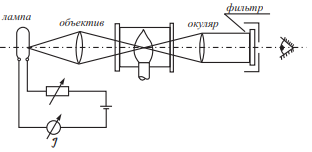
\includegraphics[width = 0.7\textwidth]{MSS-1-4}
		\caption{Измерение температуры методом обращения спектральных линий}
	\end{center}
\end{figure}

\par Схема измерения температуры пламени \textit{методом обращения спектральных линий} сходная с только что описанной.
\par Так как нагретые газы чаще всего оптически прозрачны, будем искать температуру примесей атомов дуплета натрия, которые будут находиться в термодинамическом равновесии с нашим газом.
\par Изменяя ток на фотометрической лампе добьёмся уравнивания интенсивностей излучения лампы и фотометрической лампы. Этому равенству соответствует равенство (18):

\begin{equation}
B_{\lambda}(T_b) = B_{\lambda}(T_b)e^{-k_{\lambda}L} + (1 - e^{-k_{\lambda}L})B_{\lambda}(T)
\end{equation}
где $T_b$ - яркостная температура лампы, T - яркостная температура частиц дуплета натрия в пламени, $k_{\lambda}$ - спектральный коэффициент поглощения пламени при температуре T, L - толщина излучающего слоя пламени

\par Решением этого уравнения будет равенство

\begin{equation}
T_b = T
\end{equation}

\par В реальных измерительных системах фильтр на рис. 4 заменяется спектральным прибором, позволяющим разложить излучение в спектр (монохроматором). Излучение пламени и лампы просвечивания фокусируется на входную щель монохроматора, и после прохождения излучения через диспергирующий элемент внутри монохроматора на выходе наблюдают спектр. В этом спектре видны вертикальные линии, соответствующие спектральным линиям излучения примеси, и фон от ленты фотометрической лампы, излучающей сплошной спектр. Увеличивая ток через лампу можно наблюдать, что яркие вначале по отношению к фону линии затем наоборот станут темнее фона. От этого и идет название метода — метод обращения спектральных линий.
\par Яркостная температура ленты фотометрической лампы, соответствующая обращению спектральных линий, может быть измерена пирометром как это описано выше

\section{Результаты измерений и обработка данных}

\par Определим итоговую формулу, по которой можно выразить истинную температуру пламени.
\par Введем обозначения:
\begin{itemize}
\item $T_b^{r}$, $T_b^{y}$ и $T_b^{D}$ - видимая температура вольфрамовой нити в фотометрической лампе в красном и желтом диапазонах и натрия в пламени соответственно
\item $T^W$ и $T^{D}$ - истинная температура вольфрамовой нити в фотометрической лампе и натрия в пламени (температура пламени) соответственно
\item $\lambda_{r}$ и $\lambda_{y}$ - длина волны вольфрама при температуре $T^W$ и натрия соответственно
\item $\varepsilon_{W}$ и $\varepsilon_{y}$ - степень черноты вольфрама при температуре $T^W$ и натрия соответственно (усредненные по диапазону)

\end{itemize}

\par С помощью пирометра получим видимую температуру нити фотометрической лампы. Из (17):

\begin{equation}
\frac{1}{T^W} = \frac{1}{T_b^r}+\frac{\lambda_r}{C_2}\ln{\tilde{
\varepsilon}_r}
\end{equation}

\par Видимая температура нити и натрия в желтом диапазоне равны. Из (17) и (19) получим выражения для этих температур

\begin{equation}
\frac{1}{T^W} = \frac{1}{T_b^D}+\frac{\lambda_y}{C_2}\ln{\tilde{
\varepsilon}_y}
\end{equation}

\par Выражая из (20) и (21) итоговое значение $T^D$

\begin{equation}
\frac{1}{T^D} = \frac{1}{T_b^r}+\frac{\lambda_r}{C_2}\ln{\tilde{
\varepsilon}_r} - \frac{\lambda_y}{C_2}\ln{\tilde{
\varepsilon}_y}
\end{equation}


\begin{figure}[H]
	\begin{center}
		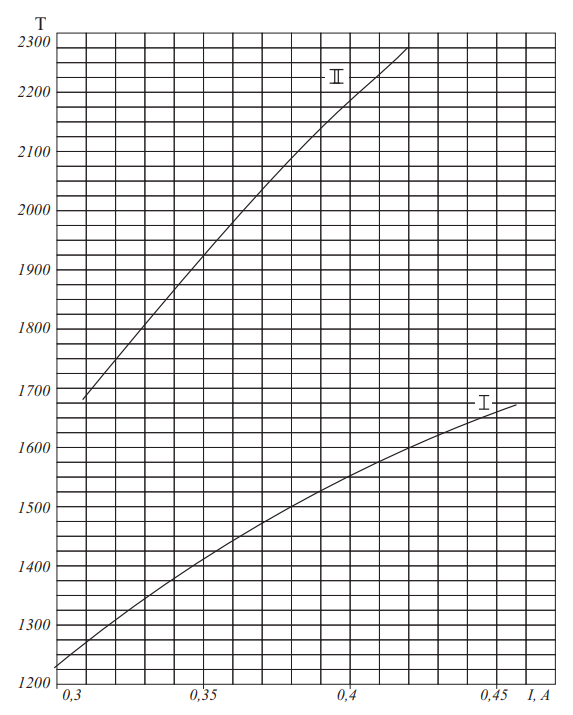
\includegraphics[width = 0.55\textwidth]{MSS-1-5}
		\caption{Тарировочные кривые для определения яркостной температуры при работе с пирометром ЛОП-72.}
	\end{center}
\end{figure}

\begin{figure}
\begin{center}
\begin{tabular}{|c|c|c|c|}
\hline 
№ измерения & 1 & 2 & 3 \\ 
\hline 
I, А & 0,34 & 0,345 & 0,355 \\ 
\hline 
$T_b^r$, K & $1865 \pm 15$ & $1900 \pm 15$ & $1950 \pm 15$ \\ 
\hline 
$T^D$, K & $1890 \pm 15$ & $1930 \pm 15$ & $1980 \pm 20$ \\ 
\hline 
\end{tabular} 
\caption{Экспериментальные значения}
\end{center}
\end{figure}

\begin{figure}[H]
	\begin{center}
		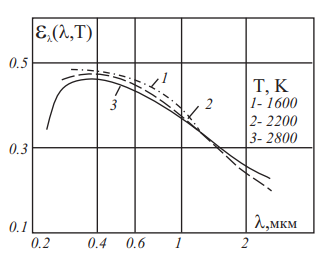
\includegraphics[width = 0.8\textwidth]{MSS-1-6}
		\caption{Тарировочные кривые для определения яркостной температуры при работе с пирометром ЛОП-72.}
	\end{center}
\end{figure}

\par Здесь для подсчетов использовались значения $\lambda_y = $ 589 нм, $\varepsilon_y = $ 0,44, $\lambda_r = $ 650 нм, $\varepsilon_r = $ 0,4
\section{Заключение}

\par В ходе работы мы изучили метод обращения спектральных линий и принцип работы пирометра, с помощью чего определили температуру пламени горелки. Усредненное полученное значение получилось равным 1920 К, с расхождением между полученными результатами не более чем на 2\%, что можно списать на фактор экспериментатора. 

\end{document}